
%template setup, made it adhere to UWA standards
\documentclass[12pt, a4paper]{article}
\usepackage{graphicx}
\usepackage{amsmath}
\usepackage{url}

%fix caption formatting
\usepackage[font=small,labelfont=bf]{caption}

%slightly modified UWA setup
\setlength{\oddsidemargin}{0.5cm}
\setlength{\evensidemargin}{0.5cm}
\setlength{\topmargin}{-1.6cm}
\setlength{\leftmargin}{0.5cm}
\setlength{\rightmargin}{0.5cm}
\setlength{\textheight}{24.00cm} 
\setlength{\textwidth}{15.0cm}
\parindent 0pt
\parskip 5pt
\pagestyle{plain}


%meta info
\title{Algorithms for RNA folding}
\author{Max Ward \\
School of Computer Science \& Software Engineering \\
The University of Western Australia}
%let the date get auto generated

%author list formatter. not really needed here, but always nice to have
\newcommand{\namelistlabel}[1]{\mbox{#1}\hfil}
\newenvironment{namelist}[1]{%1
\begin{list}{}
    {
        \let\makelabel\namelistlabel
        \settowidth{\labelwidth}{#1}
        \setlength{\leftmargin}{1.1\labelwidth}
    }
  }{%1
\end{list}}



%-------------------------------------------------------------------------

\begin{document}


%title first!
\maketitle

\begin{abstract}
Ribonucleic acid (RNA) drives many biological processes. In the last decade it has become apparent that it is important in meta-genetic pathways, allowing DNA to self regulate. In addition, it has been suggested that interactions between RNAs drive developmental processes in eukaryotes. To fully understand how RNA functions, and to further elucidate its role in biology, its structure must be understood. However, conventional imaging techniques are expensive and time consuming. As a result, the algorithmic prediction of RNA structure has tangible applications in research. Many such algorithms exist. The most widespread are those that predict RNA structures by minimizing global free energy as defined by a thermodynamic model. In this report I attempt to assay the predictive power of several thermodynamically based algorithms. In addition, I empirically test the theoretical time complexity of these algorithms. I expected that newer algorithms should have better accuracy than older algorithms, however, this was not the case. While the time complexities for all tested algorithms was verified, newer algorithms appeared to have higher constant factors. In light of this data, I suggest that older algorithms are practically better, and that more research is needed to find improved algorithms.
\end{abstract}


{\bf Keywords:} Ribonucleic acid, structure, prediction, empirical, comparison.

{\bf CR Classification:} J.3 Biology and genetics.

\clearpage

%\tableofcontents
%\listoffigures
%\clearpage

\section{Introduction}
\subsection{Motivation}
Ribonucleic acid (RNA) is at the core of many biological processes. Traditionally it has been described as the messenger molecule of DNA, faithfully carrying code from DNA to the site of protein synthesis. However, in a recent landmark paper, Amaral et al. \cite{amaral2008eukaryotic} described our genome, and those of other eukaryotes, as being driven by a RNA machine. They noted that most of the eukaryote genome is transcribed into RNA, despite little of it coding for protein. It seems that much of our genome, originally called `junk DNA', codes for functional RNA molecules. These RNAs can interact with DNA, affecting gene expression. This allows DNA to essentially regulate itself. For example, Makeyev \& Maniati \cite{makeyev2008multilevel} reported that microRNAs affect the expression of genes by interfering with the translation of protein. They also argued that microRNAs, and other regulatory RNAs, explain the vast differences between organisms with similar genomes. To put this idea into perspective, we share roughly 90\% of our genes with the domestic cat \cite{pontius2007initial}. Mattick \cite{mattick2007new} has suggested that the process of development---from embryo to adult---is encoded in the interactions of such RNAs.

A widely held axiom is that chemical structure is tantamount to biological function. With increasingly important biological functions being associated with RNA, it is essential to accurately predict its structure. The purpose of this paper is to provide a survey of some widely used RNA structure prediction algorithms. In the interest of succinctness, I review only algorithms based on a thermodynamic model. Other algorithms often use machine learned parameters; these shall not be explored here as they represent fringe areas of research. In essence, all the algorithms I test take a single RNA primary sequence as input, and produce a predicted structure as output. I hypothesize that newer algorithms should have improved accuracy compared to older algorithms. In addition, I aim to empirically verify the time complexities of tested algorithms. The Zuker algorithm was the first thermodynamic algorithm to achieve usable prediction accuracy, and is the oldest algorithm I tested.

\subsection{Relevant Algorithms}
\subsubsection{The Zuker Algorithm}
In 1981 Zuker \& Stiegler \cite{zuker1981optimal}
described an algorithm that predicts RNA structures by minimizing molecular free energy. The lower free energy a molecule has, the more stable it is. Prediction is done
by applying thermodynamic rules for canonical substructures like hairpin loops, internal bulges, multiloops (also called bifurcation loops), unbonded bases, and stacked base pairs. For examples of these structures, refer to Figure \ref{fig:zuk_struct}. The Zuker algorithm uses a mutually recursive dynamic programming recurrence to achieve a relatively comprehensive scoring scheme. This is possible because RNA structures are nested, and hence substructures with minimum free energy need not be recomputed. It follows naturally that dynamic programming can then be used to find a global minimum. The thermodynamic scoring system is borrowed from the work of Studnicka et al. \cite{studnicka1978computer} who presented a
complex but theoretically similar algorithm, albeit having
much worse asymptotic and implementation complexity. It was later improved by Matthews et al. \cite{mathews1999expanded, mathews2004incorporating}. The time complexity of the Zuker algorithm is $O(n^3)$, where $n$ is the number of nucleotides in the RNA. In short, it is able to efficiently predict structures for large RNAs on modern hardware.  Because of
its efficiency, robustness, and extensibility, this method is,
even today, still the most popular available. The most widely used packages for RNA structure prediction all contain implementations of the Zuker algorithm \cite{lorenz2011viennarna, reuter2010rnastructure}.

\begin{figure}
\begin{center}
\scalebox{0.27}{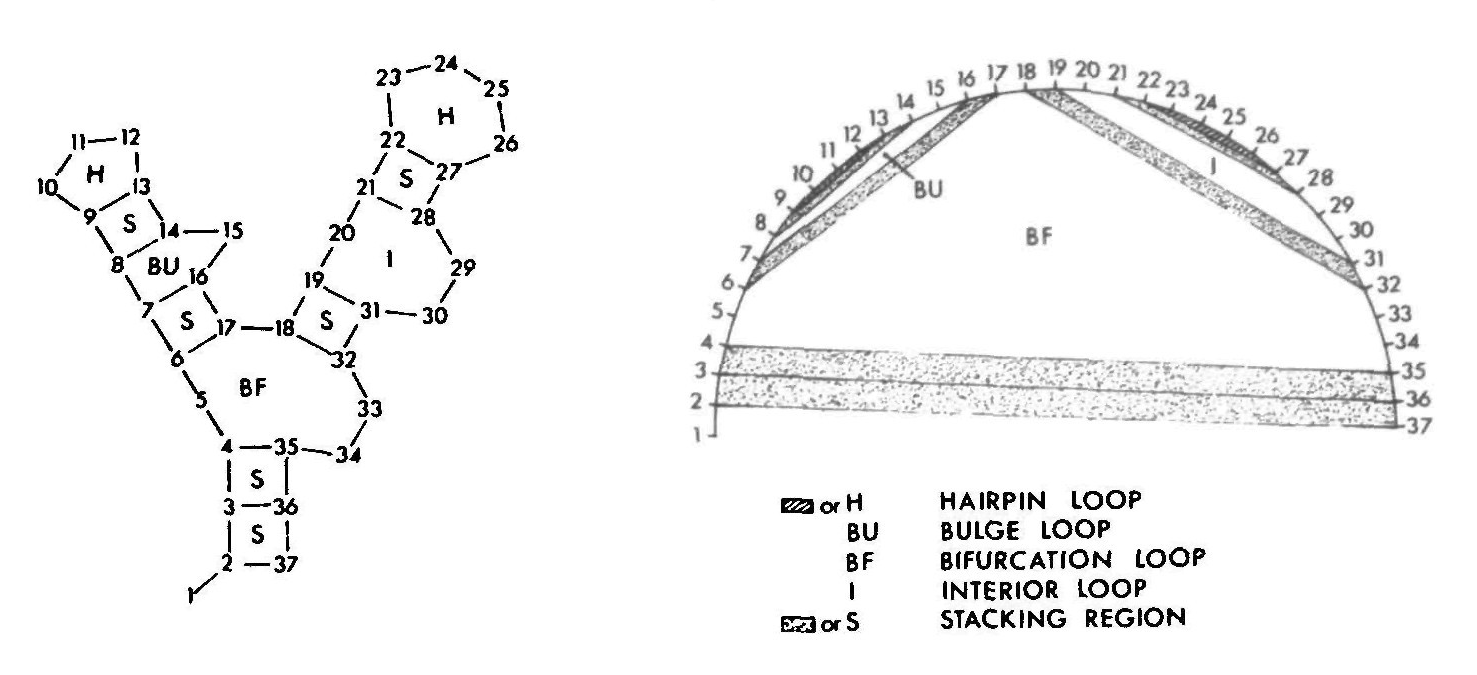
\includegraphics{figure4}}
\end{center}
\caption{Substructures used in the Zuker algorithm. On the left is a diagram of a RNA structure. On the right is the same structure laid out on a semi-circle. Bonds are represented as lines crossing the semi-circle. Taken from original
publication \cite{zuker1981optimal}.}
\label{fig:zuk_struct}
\end{figure}

\subsubsection{Maximum Expected Accuracy}
The Maximum Expected Accuracy (MEA) technique for RNA prediction was first applied by Do, Woods \& Batzoglou \cite{do2006contrafold} as part of the CONTRAfold algorithm in 2006. It is more recent than the Zuker method, and was the second class of algorithm I tested. The Zuker algorithm essentially finds the most likely structure under a thermodynamic model. The MEA prediction method is more compromising; it finds a structure containing the most probable set of bonds. This is done by computing the partition function for a RNA as described by McCaskil \cite{mccaskill1990equilibrium}. The partition function computation is achieved by a modified version of the Zuker algorithm, and can be done in $O(n^3)$ time. This is generally the most expensive step in any MEA algorithm, and hence such methods have a time complexity of $O(n^3)$. It should be noted that the this computation uses the underlying thermodynamic model of the Zuker algorithm. This partition function can be processed to produce a two dimensional matrix of base pairing probabilities. Each pair of indexes in the matrix represents the probability that the bases corresponding to those indexes will bond. Intuitively this represents the entire folding landscape of a RNA, rather than a single minimum free energy structure as computed by the Zuker algorithm. A MEA algorithm builds a structure by selecting bonds from this bond probability matrix. However, if the sum probability is naively maximized, it tends to produce structures with too many bonds. As such, a MEA algorithm must find a compromise between the number of bonds selected, and the total probability of the computed structure. Usually this is achieved by introducing some cut-off value, or, in the case of CONTRAfold, a scaling factor.

\subsubsection{Cotranscriptional Folding}
There is compelling evidence that RNA structures form during transcription. Put plainly, RNA structures begin to form before the molecule has been fully assembled. This thesis is called `cotranscriptional folding'. Kramer \& Mills \cite{kramer1981secondary} reported seeing preliminary structures form, break apart, and reform into other structures during transcription. Over a decade later, Morgan \& Higgs \cite{morgan1996evidence} examined many RNA molecules and found that typical structures have suboptimal free energy. They postulated that this is due to cotranscriptional folding. Recently, Proctor \& Meyer \cite{proctor2013cofold} purportedly improved prediction accuracy by simulating cotranscriptional folding in an algorithm they called `CoFold'. They captured the effects of cotranscriptional interactions using a scaling function, in which closer nucleotides are weighted higher than distant nucleotides. Proctor \& Meyer \cite{proctor2013cofold} reported that this improved prediction accuracy; particularly for RNA molecules comprising greater than 1000 nucleotides. CoFold extends the Zuker algorithm by injecting the aforementioned scaling function into the recurrence relation. As such, it also has a $O(n^3)$ time complexity. CoFold was the third algorithm chosen for testing.

\section{Materials and Methods}
\subsection{Environment and Software}
All software was run on the Debian 7.5 "wheezy" operating system using the default configuration. Debian was run on top of an Intel i7-4770k processor with 32 gigabytes of RAM. The GNU C Compiler version 4.8.2 was used to compile all the required code. Though the processor used was multicore, OpenMP was disabled at compile time to prevent the use of multiple cores during testing. The source code for all the algorithms tested was compiled using makefiles provided as part of their source. The latest version of the ViennaRNA suite \cite{lorenz2011viennarna} (version 2.1.7, released April 13th 2014 \cite{lorenz2014online}) was used as the reference implementation of a MEA algorithm and the Zuker algorithm. This was because it contains widely used versions of both. The module in ViennaRNA that implements the Zuker algorithm is called RNAfold, and I shall hereafter refer to it as such. Likewise, the module for MEA is simply called MEA. The entire ViennaRNA suite was compiled from source, then was linked as a static library at compile time for testing. The latest version of CoFold was downloaded from the CoFold webserver \cite{cofold2014online}. Because CoFold is based on an older version of RNAfold, it was compiled separately, and linked as a separate static library. In addition, the GNU Regression, Econometrics, and Time-series Library \cite{baiocchi2003gretl} was used for all statistical tests, and to produce accompanying graphics.

\subsection{Data Set}
The RNA structures used to test algorithms presented in this paper were taken from the RNA STRAND database \cite{andronescu2008rna}. The RNA STRAND database is a free-to-use, curated collection of RNA structures taken from various publicly available databases and publications. A subset of RNA structural data was extracted from the database. This subset contained only RNA structures that were marked as having been verified using X-ray crystallography, or nuclear magnetic resonance imaging. It also comprises only whole RNAs; none of the RNAs used were fragments or subsequences of larger RNA molecules. Finally, no duplicates were allowed in the selected set. Hereafter, I shall refer to this collection of RNA structures as the `testing set'. The testing set contained 392 different RNA molecules ranging in length from 20 to 3032 nucleotides.

\subsection{Accuracy}
Well established procedures have been developed over
the history of RNA structure prediction for comparing accuracy. Usually accuracy is determined by comparing predicted structures to known
structures. True Positives ($TP$) is defined as the number of base pairs which appear in both the predicted structure and the actual structure. False Positives
($FP$) is the number of predicted base pairs not in the true
structure \cite{lorenz2011viennarna}. Similarly, False Negatives ($FN$) is defined as the number of base
pairings in the reference structure but not present in the predicted structure \cite{lorenz2011viennarna}.
Sensitivity, also called the True Positive Rate ($TPR$), can be defined using the previously introduced values. I have given a mathematical definition of $TPR$ in Equation \ref{eq:tpr}.

\begin{equation} \label{eq:tpr}
 \frac{TP}{TP + FN}
\end{equation}

Precision, also known as Positive Predictive Value ($PPV$), can also be calculated
using these values (see Equation \ref{eq:ppv}).


\begin{equation} \label{eq:ppv}
 \frac{TP}{TP + FP}
\end{equation}

For the results presented in this report, F-score was used as a measure of accuracy. F-score is defined as the harmonic mean of sensitivity and precision. It provides a good balance between these two metrics.

\section{Results}
\label{sec:results}
\subsection{Accuracy}
To compare the accuracy of the selected algorithms, I ran each of them using the testing set as input. The structures computed by each algorithm were then compared to actual, experimentally determined structures for the corresponding RNAs, and an F-score was computed. A summary of recorded F-scores is shown graphically in Figure \ref{fig:boxplots}. In addition, summary statistics can be found in Table \ref{tab:summarystats}. A more fine grained comparison was achieved by using the Wilcoxon signed-rank test. This statistical test was chosen over the more standard t-test because the data was not normally distributed, and the Wilcoxon signed-rank test is less sensitive to non-parametric variables. A Wilcoxon signed-rank test compares the difference between samples from the same population. In our case, the sample refers to the algorithm used, and the population is the testing set, which was the same for all algorithms. Hence the assumptions of the test are satisfied. The test was run to compare each pair of algorithms. A summary of these results can be found in Table \ref{tab:wilcoxon}. Becuase none of the results were statistically significant ($p > 0.05$), we cannot reject the null hypothesis of the Wilcoxon signed-rank test. Specifically, the null hypothesis is that any difference in the compared samples is due to chance. To test the claim that CoFold is more accurate for larger RNA, the Wilcoxon signed-ranks test was repeated for only RNAs larger than 1000 nucleotides. Again the results were not statistically significant ($p > 0.05$), and the null hypothesis cannot be rejected (see Table \ref{tab:wilcoxon_large}).

\begin{figure}
\begin{center}
\scalebox{0.7}{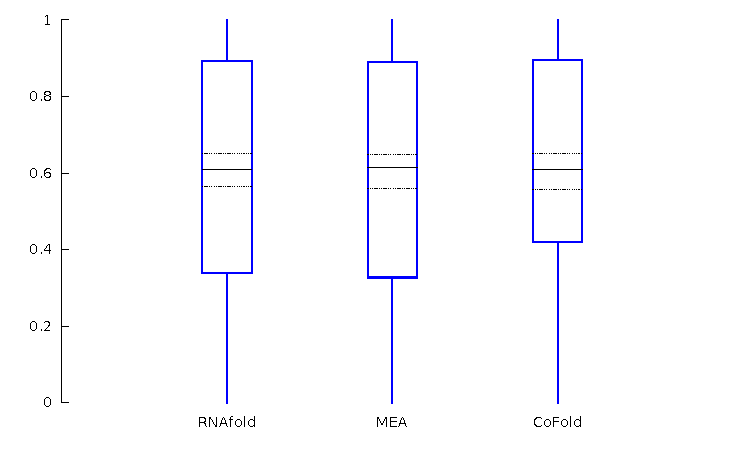
\includegraphics{boxplots}}
\end{center}
\caption{Boxplots depicting the spread of F-scores for RNAfold, MEA, and CoFold. F-scores can range from \texttt{0.0} to \texttt{1.0} as displayed on the y-axis. The tails of boxplots indicate total F-score range. Boxed area indicates interquartile range, central line indicates median value.}
\label{fig:boxplots}
\end{figure}


\begin{table}
\centering
\begin{tabular}{l*{6}{c}r}
Algorithm	& Mean & Median & Std. Dev. \\
\hline
RNAfold &  0.574834    &    0.608696 & 0.341977   \\
MEA & 0.564584    &    0.615385  & 0.346070\\
CoFold & 0.580802  &     0.608696 & 0.337973  \\
\end{tabular}
\caption{Summary statistics for the F-scores of RNAfold, MEA, and CoFold.}
\label{tab:summarystats}
\end{table}


\begin{table}
\centering
\begin{tabular}{l*{6}{c}r}
Algorithms	& $z$-value & $p$-value \\
\hline 
MEA \& CoFold &  -0.225675    &    0.410727   \\
RNAfold \& CoFold &  -0.85571    &    0.196079  \\
\end{tabular}
\caption{The results of Wilcoxon signed-rank tests for CoFold versus other algorithms using only RNA $> 1000$ nucleotides in length. The $z$-value indicates the magnitude of difference between population F-scores. The $p$-value indicates statistical significance.}
\label{tab:wilcoxon_large}
\end{table}


\begin{table}
\centering
\begin{tabular}{l*{6}{c}r}
Algorithms	& $z$-value & P-value \\
\hline 
MEA \& CoFold &  -0.97557    &    0.164639   \\
RNAfold \& CoFold &  -0.284113    &    0.388162  \\
RNAfold \& MEA &  0.290959   &    0.385541  \\
\end{tabular}
\caption{The results of Wilcoxon signed-rank tests between RNAfold, MEA, and CoFold. The $z$-value indicates the magnitude of difference between population F-scores. The $p$-value indicates statistical significance.}
\label{tab:wilcoxon}
\end{table}


\subsection{Time}

\begin{figure}
\begin{center}
\scalebox{0.8}{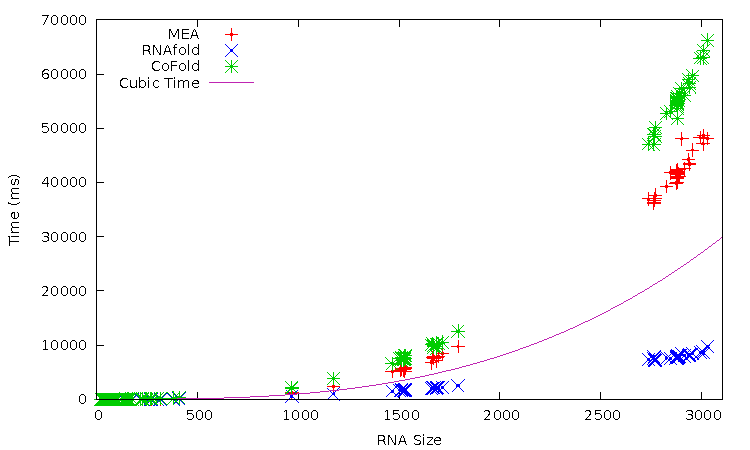
\includegraphics{timegraph}}
\end{center}
\caption{Here the recorded run time for RNAfold, MEA, and CoFold are depicted as a scatter plot. The time used by all algorithms increases with increasing RNA length. The length of a RNA is defined as the number of nucleotides it compromises. A purple line representing a generic cubic curve is included for comparison.}
\label{fig:timegraph}
\end{figure}


\begin{figure}
\begin{center}
\scalebox{0.8}{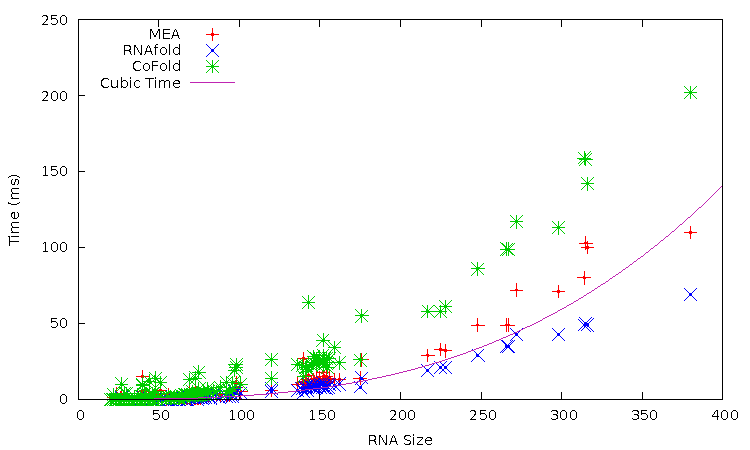
\includegraphics{timegraphsmall}}
\end{center}
\caption{Here the recorded run time for only smaller RNAs ($< 400$ nucleotides) are depicted as a scatter plot. A purple line representing a generic cubic curve is included for comparison.}
\label{fig:timegraphsmall}
\end{figure}

One of the aims of this investigation was to validate the time complexity claims of the chosen algorithms. All tested algorithms have a claimed worst case time complexity of $O(n^3)$ where $n$ is the length of the input RNA sequence. To test this, all algorithms were run using RNAs in the testing set as input. Only the time used by the algorithm was recorded, input, output, and configuration were not measured. The recorded times are presented in Figure \ref{fig:timegraph}. Because the testing set contained a large range of data, I have also included Figure \ref{fig:timegraphsmall}. This is so that run-times for smaller RNAs can be seen clearly.



\section{Discussion and Conclusions}
I have made the conjecture that newer algorithms should be more accurate at predicting RNA structures. The algorithms I have tested, in decreasing order of age, were the Zuker algorithm, MEA based algorithms, and CoFold. I ran several statistical tests to compare the F-scores of these algorithms. In every test, no statistically significant difference was found. There are only two reasonable conclusions, that the testing set was insufficiently large, or that no algorithm is significantly more accurate than the others. The testing set was large (392 RNAs), and varied, with many different classes of RNAs represented. As such, I submit that there is little difference in the predictive power of the algorithms tested. Unfortunately I was only able to test a very sparse collection of RNA prediction algorithms. Having said this, the Zuker algorithm and MEA based techniques are widely used. Additionally CoFold is a new algorithm, and represents state-of-the-art. Hence, I also submit that my findings are relevant to both research and practice. Nonetheless, further investigations should use a larger collection of algorithms, and implementations. Stochastic context free grammar based methods in particular show promise. Furthermore, if a larger testing set is available, it should be used.

A secondary goal of this investigation was to test the time requirements of the selected algorithms. While MEA and CoFold appear to have much larger constant factors compared to RNAfold, they all have a curve that is visibly cubic. This supports claims of asymptotic complexity. The Zuker algorithm has had decades of optimization, and the RNAfold implementation in particular is well optimized. As such, this may be partly an optimization discrepancy. A more detailed investigation might compare naive and optimized implementations of RNA folding algorithms.

I had supposed that one would see a progression of accuracy with newer algorithms. This was not the case. Despite this, increasingly large constant factors are evident in newer algorithms. These findings constitute compelling evidence that little progress is being made in algorithmic RNA prediction. Unfortunately, it is increasing clear that RNA has a complex and fundamental role in biology. For the time being, the most practical algorithm appears to be the Zuker algorithm---as implemented in RNAfold. It provides the best balance between predictive power and run-time efficiency. However, better algorithms are an excellent direction for future research, as better predictive power will be invaluable for understanding RNA.



%let bibtex do all the hard work
\bibliographystyle{plain}
\bibliography{assignment_three}


\end{document}

